\section{Deployment in California}\label{sec:architecture}

\begin{figure}[h]
    \centering
    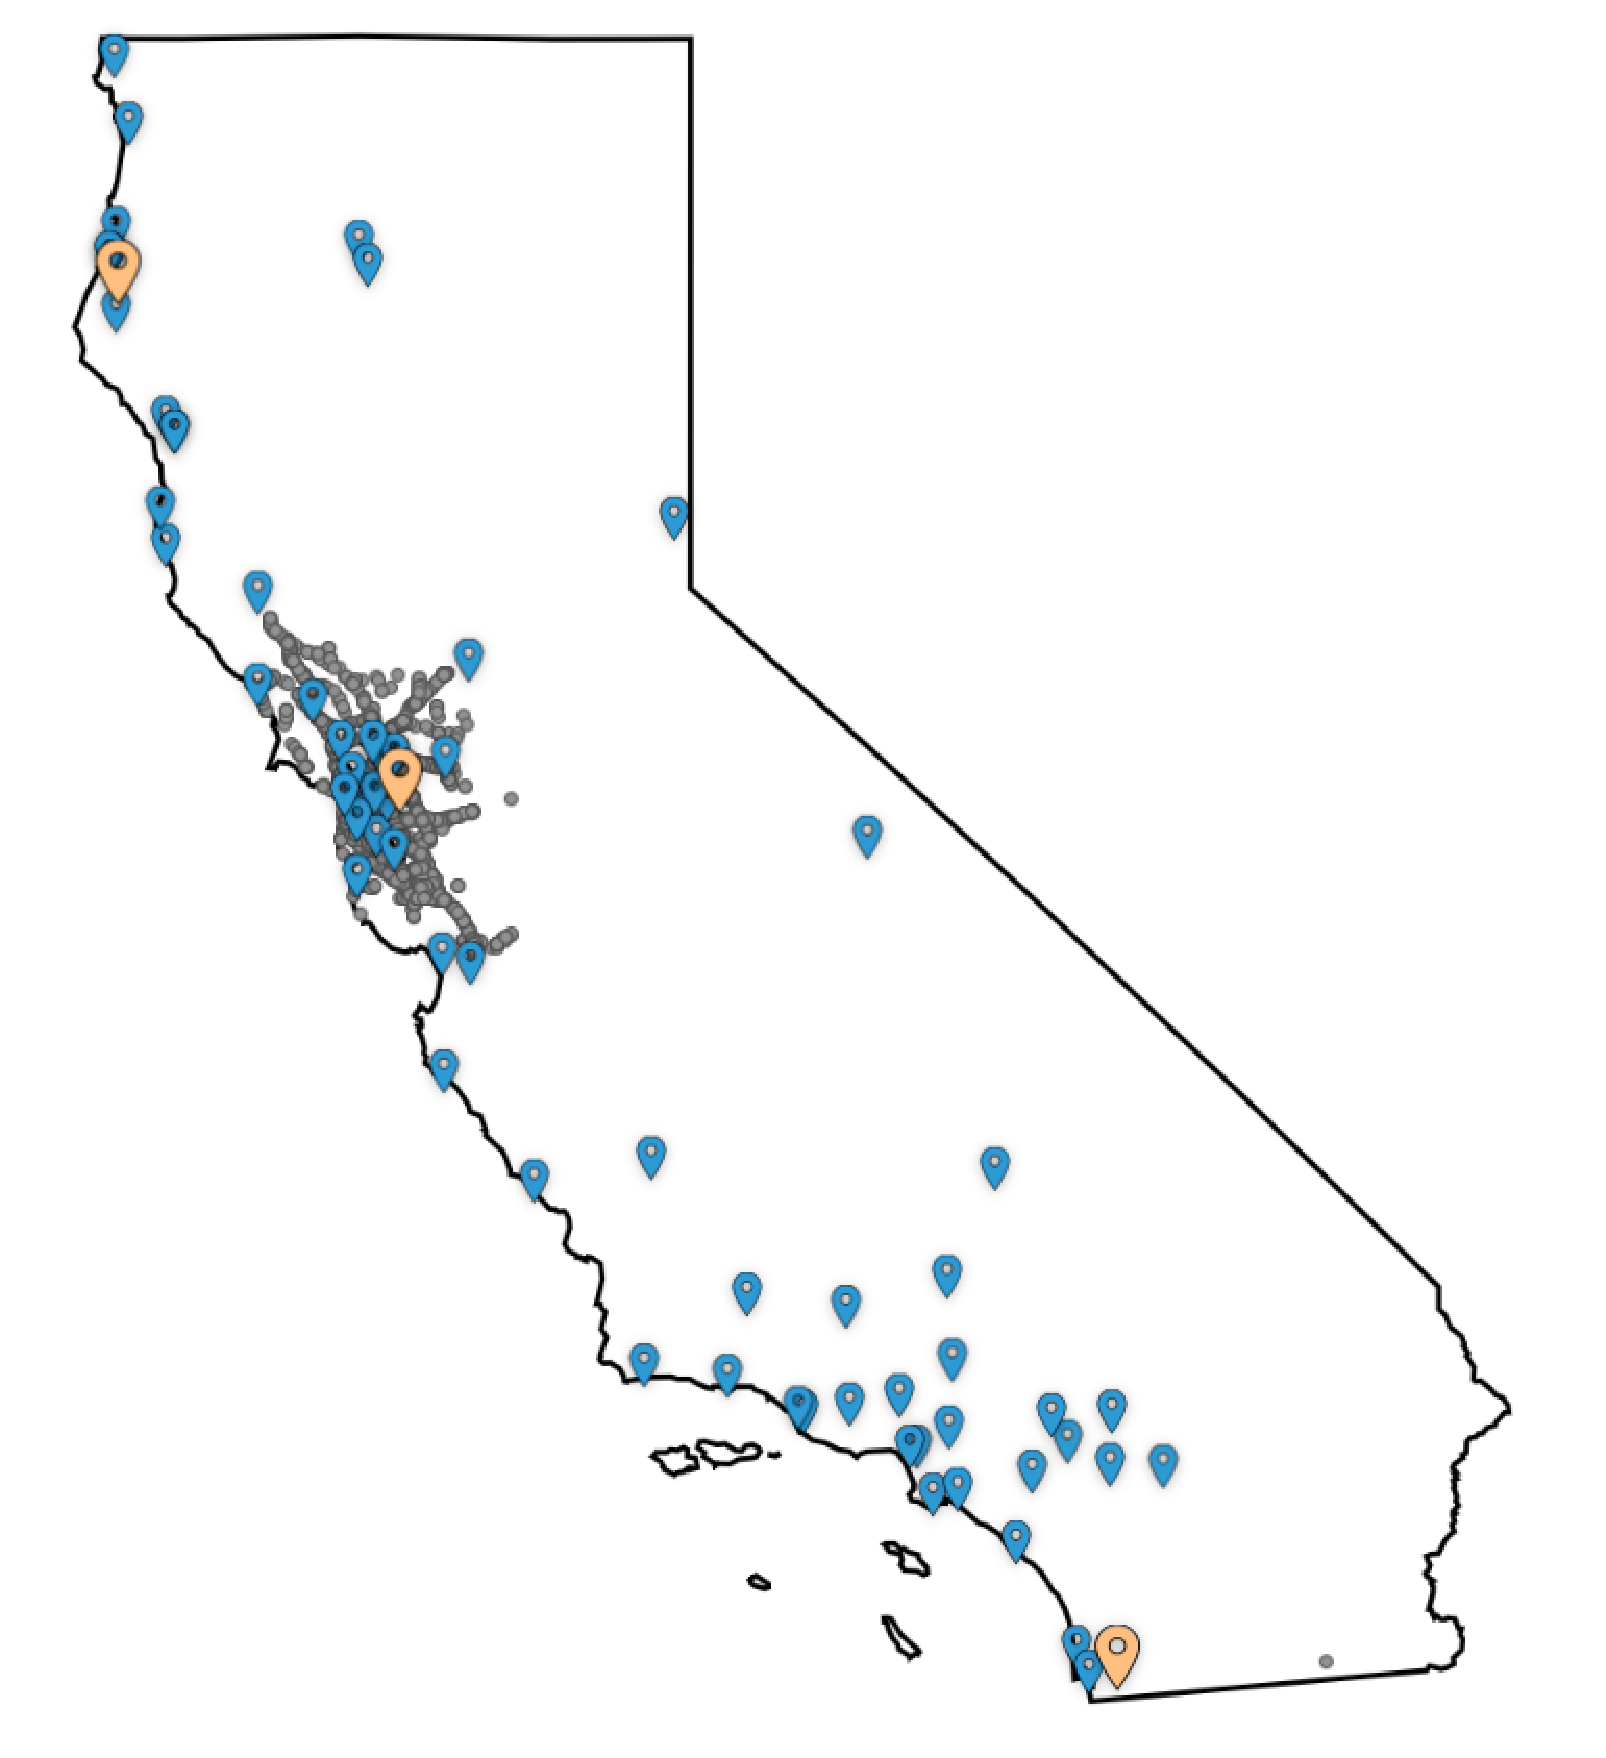
\includegraphics[width=0.5\linewidth]{Body/Irie/Figures/BridgeMap.pdf}
    \caption{Caption}
    \label{fig:placeholder}
\end{figure}

The platform was initially deployed in a 6-month pilot phase, where digital twins were created for 22 instrumented bridges in the Caltrans inventory (\cref{tab:pilots}). 
In this period, real-time monitoring was performed on the \emph{Hayward Hwy 580-238 Interchange} (CSMIP station \texttt{CE58658}), while the remaining 21 bridges where studied using preexisting records.
Following the success of this trial deployment, development of the platform was resumed with future work expected to expand its coverage of the California highway network.

\begin{table} %[h!]
\centering
    \caption{Bridges included in the pilot study for the \BRACE{} platform.}
\begin{tabular}{lllrrr}
\toprule
  \textbf{CESMD} & \textbf{Name} & \textbf{Events} & \textbf{Sensors}  & \textbf{Predictors} \\
    \midrule
    \texttt{CE13705} & Corona - I15/Hwy91 Interchange Bridge       &   3  &   9 & 6  \\ % &    \\
    \texttt{CE13795} & Capistrano Beach - I5/Via Calif. Bridge     &   5  &  12 & 3  \\ % & 5  \\
    \texttt{CE14406} & Los Angeles - Vincent Thomas Bridge         &   7  &  26 & 4  \\ % & 7  \\
    \texttt{CE24694} & Sylmar - I5/14 Interchange Bridge           &   2  &  42 & 2  \\ % & 2  \\
    \texttt{CE24704} & Los Angeles - I10/La Cienega Bridge         &   5  &  15 & 3  \\ % & 5  \\
    \texttt{CE24706} & Palmdale - Hwy 14/Barrel Springs Bridge     &   6  &  12 & 3  \\ % & 6  \\
    \texttt{CE24775} & Grapevine - I5/Lebec Rd Bridge              &   7  &  16 & 3  \\ % & 6  \\
    \texttt{CE33742} & Ridgecrest - Hwy 395/Brown Road Bridge      &   5  &   9 & 3  \\ % & 5  \\
    \texttt{CE47315} & San Juan Bautista - Hwy 101/156 Overpass    &  10  &  15 & 3  \\ % & 10  \\
    \texttt{CE68184} & Vallejo - Carquinez/I80 East Bridge         &   3  &  58 & 2  \\ % \\
    \texttt{CE68185} & Vallejo - Carquinez/I80 West Bridge         &   5  & 103 & 5  \\ % \\
    \texttt{CE79421} & Leggett - Hwy 101/Confusion Hill Bridge     &   5  &  24 & 6  \\ % \\
    \texttt{CE89686} & Eureka - Samoa Channel Bridge               &  18  &  27 & 4  \\ % \\
    \texttt{CE89708} & Arcata - Hwy 101/Murray Road Bridge         &   7  &  12 & 6  \\ % \\
    \texttt{CE89735} & Eureka - Middle Channel Bridge              &  14  &   9 & 3  \\ % \\
    \texttt{CE89736} & Eureka - Eureka Channel Bridge              &  13  &  12 & 4  \\ % \\
    \texttt{CE89973} & Rio Dell - Hwy 101/Eel River Bridge         &  44  &  18 & 3  \\ % \\
    \texttt{CE23631} & San Bernardino - I10/215 Interchange        &   9  &  18 & 4  \\ % & 9  \\
    \texttt{CE54730} & Lake Crowley - Hwy 395 Bridge               &   5  &   9 & 6  \\ % \\
    \texttt{CE89324} & Rio Dell - Hwy 101/Painter St. Overcrossing &  31  &  20 & 6  \\ % \\
    \texttt{CE01336} & Hwy8/Meloland Overpass                      &  13  &  32 & 7  \\ % & 13 \\
    \texttt{CE58658} & Hayward Hwy 580-238 Interchange             &  62  &  20 & 7  \\ % \\
\midrule
\textbf{Total} & & & 279 & 518 & 93 \\
\bottomrule
\end{tabular}
\label{tab:pilots}
\end{table}

% Structural vibration sensing and data streaming in California has seen technological developments and investments in recent years. To help monitor the state transportation network, acceleration response records are streamed from discrete locations on highway bridges that are at risk of structural damage or play a key role as recovery routes or lifelines. An ongoing research question is how to best utilize these data to monitor the health of the bridges.

% A complete framework is being developed that allows advanced state-of-the-art methodologies from disciplines like monitoring, assessment, and identification to be linked together in new, and exciting ways. 
% Considerable time and effort has been put into ensuring that the design of the framework is (1) able to remain relevant as progress continues to be made in these fields, and (2) provides a connection between these fields that is able to facilitate new and useful conclusions. Because of the novelty provided by this unique arrangement of tools, the \BRACE{} project sits at a vantage point from which several new possibilities exist for reaching new understandings in the interdisciplinary realm of seismic structural health monitoring.


\begin{figure}
    \centering
    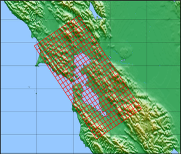
\includegraphics[width=0.5\linewidth]{Body/Irie//Figures/SGMD.png}
    \caption{Enter Caption}
    \label{fig:sgmd}
\end{figure}
\begin{Note}

An example of how SGMD \cite{mccallen2025open-access} can be leveraged to advance structural resilience research is through its integration with existing structural health monitoring platforms.

As a practical application of these advancements, integrating SGMD with \BRACE{} can significantly enhance structural health monitoring efforts. 

Data driven methods are currently limited by data sparsity, particularly for structures without instrumentation. 
Integrating SGMD with \BRACE{} addresses this limitation by enabling preemptive analysis through simulated ground motions. 
This integration allows for predictive modeling for structures lacking sensor data, improving the ability to forecast structural responses during future seismic events. Additionally, SGMD data can inform real-time assessments by providing baseline models against which real-time sensor data can be compared, enhancing the accuracy of structural health evaluations. 
This integration extends the benefits of \BRACE{} to a broader range of infrastructure within the transportation network, contributing to more comprehensive community resilience.
\end{Note}